%% document class file for the preparation of a paper
%% for the International Conference ICCAS 2020
%% global option 'fleqn' ensures equations flush left.
%% set '10pt' and 'twocolumn' options.

\documentclass[10pt,twocolumn]{ICCAS}
 
%%%%%%% set heading and page number hear %%%%%%%%%%
% % Do not put page numbers for submission.
%\setcounter{page}{101}

\usepackage{diagbox}
\usepackage{subcaption}
\usepackage[hyphens]{url}  % Allows line breaks at hyphens
\usepackage[colorlinks]{hyperref}
\usepackage{array,tabularx}
\usepackage{multicol} 
\usepackage{multirow}
\usepackage{empheq}

\usepackage{amsmath, amssymb}

\begin{document}

\newcommand{\getErrorResult}[5]{\csname#1#2#3#4#5\endcsname}
\newcommand{\FlatodometryControllerVelerrorEstimateNormMeanabs}{0.034}
\newcommand{\FlatodometryControllerVelerrorEstimateNormStd}{0.033}
\newcommand{\FlatodometryControllerVelerrorEstimateXyMeanabs}{0.030}
\newcommand{\FlatodometryControllerVelerrorEstimateXyStd}{0.030}
\newcommand{\FlatodometryControllerVelerrorEstimateZMeanabs}{0.013}
\newcommand{\FlatodometryControllerVelerrorEstimateZStd}{0.021}
\newcommand{\FlatodometryControllerVelerrorLlveNormMeanabs}{0.034}
\newcommand{\FlatodometryControllerVelerrorLlveNormStd}{0.033}
\newcommand{\FlatodometryControllerVelerrorLlveXyMeanabs}{0.030}
\newcommand{\FlatodometryControllerVelerrorLlveXyStd}{0.030}
\newcommand{\FlatodometryControllerVelerrorLlveZMeanabs}{0.013}
\newcommand{\FlatodometryControllerVelerrorLlveZStd}{0.022}
\newcommand{\FlatodometryHartleyVelerrorEstimateNormMeanabs}{0.017}
\newcommand{\FlatodometryHartleyVelerrorEstimateNormStd}{0.015}
\newcommand{\FlatodometryHartleyVelerrorEstimateXyMeanabs}{0.015}
\newcommand{\FlatodometryHartleyVelerrorEstimateXyStd}{0.015}
\newcommand{\FlatodometryHartleyVelerrorEstimateZMeanabs}{0.006}
\newcommand{\FlatodometryHartleyVelerrorEstimateZStd}{0.009}
\newcommand{\FlatodometryHartleyVelerrorLlveNormMeanabs}{0.092}
\newcommand{\FlatodometryHartleyVelerrorLlveNormStd}{0.142}
\newcommand{\FlatodometryHartleyVelerrorLlveXyMeanabs}{0.090}
\newcommand{\FlatodometryHartleyVelerrorLlveXyStd}{0.141}
\newcommand{\FlatodometryHartleyVelerrorLlveZMeanabs}{0.011}
\newcommand{\FlatodometryHartleyVelerrorLlveZStd}{0.019}
\newcommand{\FlatodometryTiltVelerrorEstimateNormMeanabs}{0.019}
\newcommand{\FlatodometryTiltVelerrorEstimateNormStd}{0.019}
\newcommand{\FlatodometryTiltVelerrorEstimateXyMeanabs}{0.018}
\newcommand{\FlatodometryTiltVelerrorEstimateXyStd}{0.018}
\newcommand{\FlatodometryTiltVelerrorEstimateZMeanabs}{0.006}
\newcommand{\FlatodometryTiltVelerrorEstimateZStd}{0.010}
\newcommand{\FlatodometryTiltVelerrorLlveNormMeanabs}{0.044}
\newcommand{\FlatodometryTiltVelerrorLlveNormStd}{0.048}
\newcommand{\FlatodometryTiltVelerrorLlveXyMeanabs}{0.042}
\newcommand{\FlatodometryTiltVelerrorLlveXyStd}{0.047}
\newcommand{\FlatodometryTiltVelerrorLlveZMeanabs}{0.010}
\newcommand{\FlatodometryTiltVelerrorLlveZStd}{0.016}
\newcommand{\FlatodometryControllerRelerrorTiltMeanabs}{1.32}
\newcommand{\FlatodometryControllerRelerrorTiltStd}{2.06}
\newcommand{\FlatodometryControllerRelerrorTransxyMeanabs}{0.034}
\newcommand{\FlatodometryControllerRelerrorTransxyStd}{0.026}
\newcommand{\FlatodometryControllerRelerrorTranszMeanabs}{0.020}
\newcommand{\FlatodometryControllerRelerrorTranszStd}{0.045}
\newcommand{\FlatodometryControllerRelerrorYawMeanabs}{1.23}
\newcommand{\FlatodometryControllerRelerrorYawStd}{1.25}
\newcommand{\FlatodometryHartleyRelerrorTiltMeanabs}{1.00}
\newcommand{\FlatodometryHartleyRelerrorTiltStd}{1.84}
\newcommand{\FlatodometryHartleyRelerrorTransxyMeanabs}{0.046}
\newcommand{\FlatodometryHartleyRelerrorTransxyStd}{0.056}
\newcommand{\FlatodometryHartleyRelerrorTranszMeanabs}{0.026}
\newcommand{\FlatodometryHartleyRelerrorTranszStd}{0.051}
\newcommand{\FlatodometryHartleyRelerrorYawMeanabs}{0.96}
\newcommand{\FlatodometryHartleyRelerrorYawStd}{0.92}
\newcommand{\FlatodometryTiltRelerrorTiltMeanabs}{0.94}
\newcommand{\FlatodometryTiltRelerrorTiltStd}{1.97}
\newcommand{\FlatodometryTiltRelerrorTransxyMeanabs}{0.031}
\newcommand{\FlatodometryTiltRelerrorTransxyStd}{0.021}
\newcommand{\FlatodometryTiltRelerrorTranszMeanabs}{0.030}
\newcommand{\FlatodometryTiltRelerrorTranszStd}{0.046}
\newcommand{\FlatodometryTiltRelerrorYawMeanabs}{1.15}
\newcommand{\FlatodometryTiltRelerrorYawStd}{1.18}
\newcommand{\FlatodometryControllerAbserrorKoTrobobdRhpsaATiltMeanabs}{1.08}
\newcommand{\FlatodometryControllerAbserrorKoTrobobdRhpsaATiltStd}{0.43}
\newcommand{\FlatodometryControllerAbserrorKoTrobobdRhpsaATransxyMeanabs}{0.236}
\newcommand{\FlatodometryControllerAbserrorKoTrobobdRhpsaATransxyStd}{0.144}
\newcommand{\FlatodometryControllerAbserrorKoTrobobdRhpsaATranszMeanabs}{0.002}
\newcommand{\FlatodometryControllerAbserrorKoTrobobdRhpsaATranszStd}{0.003}
\newcommand{\FlatodometryControllerAbserrorKoTrobobdRhpsaAYawMeanabs}{2.71}
\newcommand{\FlatodometryControllerAbserrorKoTrobobdRhpsaAYawStd}{3.39}
\newcommand{\FlatodometryHartleyAbserrorKoTrobobdRhpsaATiltMeanabs}{1.22}
\newcommand{\FlatodometryHartleyAbserrorKoTrobobdRhpsaATiltStd}{0.40}
\newcommand{\FlatodometryHartleyAbserrorKoTrobobdRhpsaATransxyMeanabs}{0.260}
\newcommand{\FlatodometryHartleyAbserrorKoTrobobdRhpsaATransxyStd}{0.115}
\newcommand{\FlatodometryHartleyAbserrorKoTrobobdRhpsaATranszMeanabs}{0.160}
\newcommand{\FlatodometryHartleyAbserrorKoTrobobdRhpsaATranszStd}{0.178}
\newcommand{\FlatodometryHartleyAbserrorKoTrobobdRhpsaAYawMeanabs}{5.54}
\newcommand{\FlatodometryHartleyAbserrorKoTrobobdRhpsaAYawStd}{6.12}
\newcommand{\FlatodometryTiltAbserrorKoTrobobdRhpsaATiltMeanabs}{0.96}
\newcommand{\FlatodometryTiltAbserrorKoTrobobdRhpsaATiltStd}{0.31}
\newcommand{\FlatodometryTiltAbserrorKoTrobobdRhpsaATransxyMeanabs}{0.226}
\newcommand{\FlatodometryTiltAbserrorKoTrobobdRhpsaATransxyStd}{0.128}
\newcommand{\FlatodometryTiltAbserrorKoTrobobdRhpsaATranszMeanabs}{0.225}
\newcommand{\FlatodometryTiltAbserrorKoTrobobdRhpsaATranszStd}{0.253}
\newcommand{\FlatodometryTiltAbserrorKoTrobobdRhpsaAYawMeanabs}{2.52}
\newcommand{\FlatodometryTiltAbserrorKoTrobobdRhpsaAYawStd}{3.08}
\newcommand{\FlatodometryControllerAbserrorKoTrobobdRhpsaBTiltMeanabs}{0.90}
\newcommand{\FlatodometryControllerAbserrorKoTrobobdRhpsaBTiltStd}{0.46}
\newcommand{\FlatodometryControllerAbserrorKoTrobobdRhpsaBTransxyMeanabs}{0.179}
\newcommand{\FlatodometryControllerAbserrorKoTrobobdRhpsaBTransxyStd}{0.107}
\newcommand{\FlatodometryControllerAbserrorKoTrobobdRhpsaBTranszMeanabs}{0.002}
\newcommand{\FlatodometryControllerAbserrorKoTrobobdRhpsaBTranszStd}{0.003}
\newcommand{\FlatodometryControllerAbserrorKoTrobobdRhpsaBYawMeanabs}{2.28}
\newcommand{\FlatodometryControllerAbserrorKoTrobobdRhpsaBYawStd}{3.40}
\newcommand{\FlatodometryHartleyAbserrorKoTrobobdRhpsaBTiltMeanabs}{1.11}
\newcommand{\FlatodometryHartleyAbserrorKoTrobobdRhpsaBTiltStd}{0.36}
\newcommand{\FlatodometryHartleyAbserrorKoTrobobdRhpsaBTransxyMeanabs}{0.154}
\newcommand{\FlatodometryHartleyAbserrorKoTrobobdRhpsaBTransxyStd}{0.100}
\newcommand{\FlatodometryHartleyAbserrorKoTrobobdRhpsaBTranszMeanabs}{0.154}
\newcommand{\FlatodometryHartleyAbserrorKoTrobobdRhpsaBTranszStd}{0.177}
\newcommand{\FlatodometryHartleyAbserrorKoTrobobdRhpsaBYawMeanabs}{2.05}
\newcommand{\FlatodometryHartleyAbserrorKoTrobobdRhpsaBYawStd}{1.73}
\newcommand{\FlatodometryTiltAbserrorKoTrobobdRhpsaBTiltMeanabs}{0.84}
\newcommand{\FlatodometryTiltAbserrorKoTrobobdRhpsaBTiltStd}{0.30}
\newcommand{\FlatodometryTiltAbserrorKoTrobobdRhpsaBTransxyMeanabs}{0.168}
\newcommand{\FlatodometryTiltAbserrorKoTrobobdRhpsaBTransxyStd}{0.101}
\newcommand{\FlatodometryTiltAbserrorKoTrobobdRhpsaBTranszMeanabs}{0.196}
\newcommand{\FlatodometryTiltAbserrorKoTrobobdRhpsaBTranszStd}{0.228}
\newcommand{\FlatodometryTiltAbserrorKoTrobobdRhpsaBYawMeanabs}{4.18}
\newcommand{\FlatodometryTiltAbserrorKoTrobobdRhpsaBYawStd}{4.88}
\newcommand{\FlatodometryControllerAbserrorKoTrobobdRhpsaCTiltMeanabs}{1.04}
\newcommand{\FlatodometryControllerAbserrorKoTrobobdRhpsaCTiltStd}{0.48}
\newcommand{\FlatodometryControllerAbserrorKoTrobobdRhpsaCTransxyMeanabs}{0.303}
\newcommand{\FlatodometryControllerAbserrorKoTrobobdRhpsaCTransxyStd}{0.189}
\newcommand{\FlatodometryControllerAbserrorKoTrobobdRhpsaCTranszMeanabs}{0.002}
\newcommand{\FlatodometryControllerAbserrorKoTrobobdRhpsaCTranszStd}{0.003}
\newcommand{\FlatodometryControllerAbserrorKoTrobobdRhpsaCYawMeanabs}{4.72}
\newcommand{\FlatodometryControllerAbserrorKoTrobobdRhpsaCYawStd}{5.31}
\newcommand{\FlatodometryHartleyAbserrorKoTrobobdRhpsaCTiltMeanabs}{1.01}
\newcommand{\FlatodometryHartleyAbserrorKoTrobobdRhpsaCTiltStd}{0.36}
\newcommand{\FlatodometryHartleyAbserrorKoTrobobdRhpsaCTransxyMeanabs}{0.155}
\newcommand{\FlatodometryHartleyAbserrorKoTrobobdRhpsaCTransxyStd}{0.112}
\newcommand{\FlatodometryHartleyAbserrorKoTrobobdRhpsaCTranszMeanabs}{0.150}
\newcommand{\FlatodometryHartleyAbserrorKoTrobobdRhpsaCTranszStd}{0.165}
\newcommand{\FlatodometryHartleyAbserrorKoTrobobdRhpsaCYawMeanabs}{3.05}
\newcommand{\FlatodometryHartleyAbserrorKoTrobobdRhpsaCYawStd}{3.30}
\newcommand{\FlatodometryTiltAbserrorKoTrobobdRhpsaCTiltMeanabs}{0.76}
\newcommand{\FlatodometryTiltAbserrorKoTrobobdRhpsaCTiltStd}{0.32}
\newcommand{\FlatodometryTiltAbserrorKoTrobobdRhpsaCTransxyMeanabs}{0.203}
\newcommand{\FlatodometryTiltAbserrorKoTrobobdRhpsaCTransxyStd}{0.104}
\newcommand{\FlatodometryTiltAbserrorKoTrobobdRhpsaCTranszMeanabs}{0.191}
\newcommand{\FlatodometryTiltAbserrorKoTrobobdRhpsaCTranszStd}{0.214}
\newcommand{\FlatodometryTiltAbserrorKoTrobobdRhpsaCYawMeanabs}{3.19}
\newcommand{\FlatodometryTiltAbserrorKoTrobobdRhpsaCYawStd}{3.78}
\newcommand{\FlatodometryControllerAbserrorKoTrobobdRhpsaDTiltMeanabs}{14.36}
\newcommand{\FlatodometryControllerAbserrorKoTrobobdRhpsaDTiltStd}{0.61}
\newcommand{\FlatodometryControllerAbserrorKoTrobobdRhpsaDTransxyMeanabs}{0.401}
\newcommand{\FlatodometryControllerAbserrorKoTrobobdRhpsaDTransxyStd}{0.367}
\newcommand{\FlatodometryControllerAbserrorKoTrobobdRhpsaDTranszMeanabs}{0.002}
\newcommand{\FlatodometryControllerAbserrorKoTrobobdRhpsaDTranszStd}{0.003}
\newcommand{\FlatodometryControllerAbserrorKoTrobobdRhpsaDYawMeanabs}{5.59}
\newcommand{\FlatodometryControllerAbserrorKoTrobobdRhpsaDYawStd}{7.47}
\newcommand{\FlatodometryHartleyAbserrorKoTrobobdRhpsaDTiltMeanabs}{13.18}
\newcommand{\FlatodometryHartleyAbserrorKoTrobobdRhpsaDTiltStd}{0.53}
\newcommand{\FlatodometryHartleyAbserrorKoTrobobdRhpsaDTransxyMeanabs}{0.300}
\newcommand{\FlatodometryHartleyAbserrorKoTrobobdRhpsaDTransxyStd}{0.256}
\newcommand{\FlatodometryHartleyAbserrorKoTrobobdRhpsaDTranszMeanabs}{0.162}
\newcommand{\FlatodometryHartleyAbserrorKoTrobobdRhpsaDTranszStd}{0.183}
\newcommand{\FlatodometryHartleyAbserrorKoTrobobdRhpsaDYawMeanabs}{11.91}
\newcommand{\FlatodometryHartleyAbserrorKoTrobobdRhpsaDYawStd}{12.38}
\newcommand{\FlatodometryTiltAbserrorKoTrobobdRhpsaDTiltMeanabs}{13.71}
\newcommand{\FlatodometryTiltAbserrorKoTrobobdRhpsaDTiltStd}{0.26}
\newcommand{\FlatodometryTiltAbserrorKoTrobobdRhpsaDTransxyMeanabs}{0.282}
\newcommand{\FlatodometryTiltAbserrorKoTrobobdRhpsaDTransxyStd}{0.209}
\newcommand{\FlatodometryTiltAbserrorKoTrobobdRhpsaDTranszMeanabs}{0.212}
\newcommand{\FlatodometryTiltAbserrorKoTrobobdRhpsaDTranszStd}{0.243}
\newcommand{\FlatodometryTiltAbserrorKoTrobobdRhpsaDYawMeanabs}{3.62}
\newcommand{\FlatodometryTiltAbserrorKoTrobobdRhpsaDYawStd}{4.01}
\newcommand{\FlatodometryControllerAbserrorKoTrobobdRhpsaETiltMeanabs}{1.82}
\newcommand{\FlatodometryControllerAbserrorKoTrobobdRhpsaETiltStd}{0.52}
\newcommand{\FlatodometryControllerAbserrorKoTrobobdRhpsaETransxyMeanabs}{0.238}
\newcommand{\FlatodometryControllerAbserrorKoTrobobdRhpsaETransxyStd}{0.122}
\newcommand{\FlatodometryControllerAbserrorKoTrobobdRhpsaETranszMeanabs}{0.003}
\newcommand{\FlatodometryControllerAbserrorKoTrobobdRhpsaETranszStd}{0.003}
\newcommand{\FlatodometryControllerAbserrorKoTrobobdRhpsaEYawMeanabs}{2.77}
\newcommand{\FlatodometryControllerAbserrorKoTrobobdRhpsaEYawStd}{2.01}
\newcommand{\FlatodometryHartleyAbserrorKoTrobobdRhpsaETiltMeanabs}{0.57}
\newcommand{\FlatodometryHartleyAbserrorKoTrobobdRhpsaETiltStd}{0.46}
\newcommand{\FlatodometryHartleyAbserrorKoTrobobdRhpsaETransxyMeanabs}{0.205}
\newcommand{\FlatodometryHartleyAbserrorKoTrobobdRhpsaETransxyStd}{0.104}
\newcommand{\FlatodometryHartleyAbserrorKoTrobobdRhpsaETranszMeanabs}{0.147}
\newcommand{\FlatodometryHartleyAbserrorKoTrobobdRhpsaETranszStd}{0.171}
\newcommand{\FlatodometryHartleyAbserrorKoTrobobdRhpsaEYawMeanabs}{4.26}
\newcommand{\FlatodometryHartleyAbserrorKoTrobobdRhpsaEYawStd}{4.55}
\newcommand{\FlatodometryTiltAbserrorKoTrobobdRhpsaETiltMeanabs}{1.21}
\newcommand{\FlatodometryTiltAbserrorKoTrobobdRhpsaETiltStd}{0.24}
\newcommand{\FlatodometryTiltAbserrorKoTrobobdRhpsaETransxyMeanabs}{0.197}
\newcommand{\FlatodometryTiltAbserrorKoTrobobdRhpsaETransxyStd}{0.092}
\newcommand{\FlatodometryTiltAbserrorKoTrobobdRhpsaETranszMeanabs}{0.203}
\newcommand{\FlatodometryTiltAbserrorKoTrobobdRhpsaETranszStd}{0.232}
\newcommand{\FlatodometryTiltAbserrorKoTrobobdRhpsaEYawMeanabs}{2.44}
\newcommand{\FlatodometryTiltAbserrorKoTrobobdRhpsaEYawStd}{2.37}



\newcommand{\MulticontactControllerVelerrorEstimateNormMeanabs}{0.034}
\newcommand{\MulticontactControllerVelerrorEstimateNormStd}{0.033}
\newcommand{\MulticontactControllerVelerrorEstimateXyMeanabs}{0.030}
\newcommand{\MulticontactControllerVelerrorEstimateXyStd}{0.030}
\newcommand{\MulticontactControllerVelerrorEstimateZMeanabs}{0.013}
\newcommand{\MulticontactControllerVelerrorEstimateZStd}{0.021}
\newcommand{\MulticontactControllerVelerrorLlveNormMeanabs}{0.034}
\newcommand{\MulticontactControllerVelerrorLlveNormStd}{0.033}
\newcommand{\MulticontactControllerVelerrorLlveXyMeanabs}{0.030}
\newcommand{\MulticontactControllerVelerrorLlveXyStd}{0.030}
\newcommand{\MulticontactControllerVelerrorLlveZMeanabs}{0.013}
\newcommand{\MulticontactControllerVelerrorLlveZStd}{0.022}
\newcommand{\MulticontactHartleyVelerrorEstimateNormMeanabs}{0.017}
\newcommand{\MulticontactHartleyVelerrorEstimateNormStd}{0.015}
\newcommand{\MulticontactHartleyVelerrorEstimateXyMeanabs}{0.015}
\newcommand{\MulticontactHartleyVelerrorEstimateXyStd}{0.015}
\newcommand{\MulticontactHartleyVelerrorEstimateZMeanabs}{0.006}
\newcommand{\MulticontactHartleyVelerrorEstimateZStd}{0.009}
\newcommand{\MulticontactHartleyVelerrorLlveNormMeanabs}{0.092}
\newcommand{\MulticontactHartleyVelerrorLlveNormStd}{0.142}
\newcommand{\MulticontactHartleyVelerrorLlveXyMeanabs}{0.090}
\newcommand{\MulticontactHartleyVelerrorLlveXyStd}{0.141}
\newcommand{\MulticontactHartleyVelerrorLlveZMeanabs}{0.011}
\newcommand{\MulticontactHartleyVelerrorLlveZStd}{0.019}
\newcommand{\MulticontactTiltVelerrorEstimateNormMeanabs}{0.019}
\newcommand{\MulticontactTiltVelerrorEstimateNormStd}{0.019}
\newcommand{\MulticontactTiltVelerrorEstimateXyMeanabs}{0.018}
\newcommand{\MulticontactTiltVelerrorEstimateXyStd}{0.018}
\newcommand{\MulticontactTiltVelerrorEstimateZMeanabs}{0.006}
\newcommand{\MulticontactTiltVelerrorEstimateZStd}{0.010}
\newcommand{\MulticontactTiltVelerrorLlveNormMeanabs}{0.044}
\newcommand{\MulticontactTiltVelerrorLlveNormStd}{0.048}
\newcommand{\MulticontactTiltVelerrorLlveXyMeanabs}{0.042}
\newcommand{\MulticontactTiltVelerrorLlveXyStd}{0.047}
\newcommand{\MulticontactTiltVelerrorLlveZMeanabs}{0.010}
\newcommand{\MulticontactTiltVelerrorLlveZStd}{0.016}
\newcommand{\MulticontactControllerRelerrorTiltMeanabs}{1.16}
\newcommand{\MulticontactControllerRelerrorTiltStd}{0.58}
\newcommand{\MulticontactControllerRelerrorTransxyMeanabs}{0.016}
\newcommand{\MulticontactControllerRelerrorTransxyStd}{0.008}
\newcommand{\MulticontactControllerRelerrorTranszMeanabs}{0.006}
\newcommand{\MulticontactControllerRelerrorTranszStd}{0.007}
\newcommand{\MulticontactControllerRelerrorYawMeanabs}{0.50}
\newcommand{\MulticontactControllerRelerrorYawStd}{0.35}
\newcommand{\MulticontactHartleyRelerrorTiltMeanabs}{0.57}
\newcommand{\MulticontactHartleyRelerrorTiltStd}{1.02}
\newcommand{\MulticontactHartleyRelerrorTransxyMeanabs}{0.012}
\newcommand{\MulticontactHartleyRelerrorTransxyStd}{0.016}
\newcommand{\MulticontactHartleyRelerrorTranszMeanabs}{0.004}
\newcommand{\MulticontactHartleyRelerrorTranszStd}{0.007}
\newcommand{\MulticontactHartleyRelerrorYawMeanabs}{0.47}
\newcommand{\MulticontactHartleyRelerrorYawStd}{0.65}
\newcommand{\MulticontactTiltRelerrorTiltMeanabs}{0.23}
\newcommand{\MulticontactTiltRelerrorTiltStd}{0.17}
\newcommand{\MulticontactTiltRelerrorTransxyMeanabs}{0.007}
\newcommand{\MulticontactTiltRelerrorTransxyStd}{0.005}
\newcommand{\MulticontactTiltRelerrorTranszMeanabs}{0.002}
\newcommand{\MulticontactTiltRelerrorTranszStd}{0.003}
\newcommand{\MulticontactTiltRelerrorYawMeanabs}{0.40}
\newcommand{\MulticontactTiltRelerrorYawStd}{0.32}
\newcommand{\MulticontactControllerAbserrorHrpeMulticontactATiltMeanabs}{0.99}
\newcommand{\MulticontactControllerAbserrorHrpeMulticontactATiltStd}{0.67}
\newcommand{\MulticontactControllerAbserrorHrpeMulticontactATransxyMeanabs}{0.019}
\newcommand{\MulticontactControllerAbserrorHrpeMulticontactATransxyStd}{0.008}
\newcommand{\MulticontactControllerAbserrorHrpeMulticontactATranszMeanabs}{0.004}
\newcommand{\MulticontactControllerAbserrorHrpeMulticontactATranszStd}{0.005}
\newcommand{\MulticontactControllerAbserrorHrpeMulticontactAYawMeanabs}{1.36}
\newcommand{\MulticontactControllerAbserrorHrpeMulticontactAYawStd}{0.74}
\newcommand{\MulticontactHartleyAbserrorHrpeMulticontactATiltMeanabs}{0.68}
\newcommand{\MulticontactHartleyAbserrorHrpeMulticontactATiltStd}{0.26}
\newcommand{\MulticontactHartleyAbserrorHrpeMulticontactATransxyMeanabs}{0.006}
\newcommand{\MulticontactHartleyAbserrorHrpeMulticontactATransxyStd}{0.003}
\newcommand{\MulticontactHartleyAbserrorHrpeMulticontactATranszMeanabs}{0.003}
\newcommand{\MulticontactHartleyAbserrorHrpeMulticontactATranszStd}{0.003}
\newcommand{\MulticontactHartleyAbserrorHrpeMulticontactAYawMeanabs}{1.35}
\newcommand{\MulticontactHartleyAbserrorHrpeMulticontactAYawStd}{0.67}
\newcommand{\MulticontactTiltAbserrorHrpeMulticontactATiltMeanabs}{0.34}
\newcommand{\MulticontactTiltAbserrorHrpeMulticontactATiltStd}{0.17}
\newcommand{\MulticontactTiltAbserrorHrpeMulticontactATransxyMeanabs}{0.009}
\newcommand{\MulticontactTiltAbserrorHrpeMulticontactATransxyStd}{0.003}
\newcommand{\MulticontactTiltAbserrorHrpeMulticontactATranszMeanabs}{0.004}
\newcommand{\MulticontactTiltAbserrorHrpeMulticontactATranszStd}{0.005}
\newcommand{\MulticontactTiltAbserrorHrpeMulticontactAYawMeanabs}{1.06}
\newcommand{\MulticontactTiltAbserrorHrpeMulticontactAYawStd}{0.93}

\title{{\scshape Valinor}: a Lightweight Leg Inertial Odometry for Humanoid Robots}

\author{Arnaud Demont*${}^{1,2,3}$, Mehdi Benallegue${}^{1}$, Thomas Duvinage${}^{1}$, and Abdelaziz Benallegue${}^{1,2,3}$}

% \author{First A. Author${}^{1}$ and Second B. Author${}^{2*}$ }

% \affils{ ${}^{1}$Department of Electrical Engineering, Hankook University, \\
% Seoul, 13391, Korea (first@hankook.ac.kr) \\
% ${}^{2}$Department of Mechanical Engineering, Hankook University, \\
% Seoul, 13391, Korea (second@hankook.ac.kr) {\small${}^{*}$ Corresponding author}}

\affils{
${}^{1}$CNRS-AIST JRL (Joint Robotics Laboratory), IRL, National Institute of Advanced Industrial Science and Technology,\\  Tsukuba,  305-8560 Japan (arnaud.demont@aist.go.jp, mehdi.benallegue@aist.go.jp, thomas.duvinage@aist.go.jp). \\
${}^{2}$Université Paris-Saclay,   91190 Gif-sur-Yvette, France.\\
${}^{3}$Laboratoire d'Ingénierie des Systèmes de Versailles (LISV),\\   78140 Vélizy, France (arnaud.demont@uvsq.fr, abdelaziz.benallegue@uvsq.fr). \\ {\small${}^{*}$ Corresponding author}
}


\abstract{
This article presents {\scshape Valinor} (Velocity-Aided Leg Inertial Nonlinear Odometry and Registration), a method for Leg-Inertial odometry for humanoid robots addressing the challenge of lightweight yet accurate and certifiable state estimation. {\scshape Valinor} associates Leg odometry with the Tilt Observer, a computationally efficient complementary filter, which provides accurate estimates of the IMU's tilt and linear velocity with strong mathematical convergence guarantees. We introduce an axis-agnostic method for the fusion of the Leg odometry's yaw with the Tilt Observer's tilt estimate. We argue that this method is less arbitrary and more mathematically sound than those based on other orientation representations, especially on Euler angles.
We present an evaluation of the proposed estimator through real-world data on two humanoid robots. We show that, while being 7.5 times faster than the state-of-the-art method used for comparison, {\scshape Valinor} improves tilt estimation by over 25\%, making it a well-suited feedback for balance and walking controllers. 
}

\keywords{
    Lightweight state estimation, Humanoid robots, Proprioceptive odometry, Tilt estimation, Balancing.
}

\maketitle

%-----------------------------------------------------------------------

\section{Introduction}

Humanoid robot navigation in real-world environments remains a core challenge in robotics. Deploying robots at scale in society and industry requires strong guarantees on their ability to plan motion, and execute actions in real time, in order to ensure safe, predictable, and certifiable behavior.

In the meantime, methods for motion generation continue to gain in complexity and capability. Notably, Model Predictive Control (MPC)~\cite{Dallard2024AdiosStabilizers} and reinforcement learning-based controllers~\cite{Peters2003ReinforcmentLearningForHumanoid} are becoming more prevalent due to their ability to handle long-horizon planning, complex dynamics, and to their versatility. However, these advances come at the cost of increased computational complexity, running them in real-time on resource-limited platforms like embedded systems thus becomes challenging~\cite{findeisen2004computationalDelayNMPC}. Since the control part is getting heavier, one practical solution is to reduce the computational load of other parts of the pipeline. 

The state estimation part is one of the cornerstones of the pipeline, since other components depend on its output and often have to wait for it before executing, and thus cannot run in parallel. For this reason, there is a need for lightweight state estimation methods, which focus on improving the estimation of key variables at high frequency using the proprioceptive sensors readily available on the robot. The most common sensors for humanoids are joint encoders, inertial measurement units (IMUs) and contact force sensors such as FSR or force/torque sensors.

In this work we propose {\scshape Valinor} (Velocity-Aided Leg Inertial Nonlinear Odometry and Registration), a method for Leg-Inertial odometry for legged robots, which relies on a highly accurate tilt estimate provided by a nonlinear complementary filter~\cite{benallegue2020LyapunovStableOrientationEstimatorHumanoids}. This complementary filter allows for a much faster computation than the conventionally used Kalman Filter (e.g.~\cite{Hartley2020RIEKF}), and offers mathematical convergence guarantees on the tilt and linear velocity estimate. \\
The main contributions introduced in this paper are as follows:
\begin{itemize}
  \item The proposed state estimator is 7.5 times faster than the start-of-the-art method for proprioceptive odometry, while displaying on par odometry accuracy, and even improving significantly tilt estimation.
  \item We present the axis-agnostic tilt and yaw fusion, which we show to be more mathematically sound than that based on Euler angle representations.
  \item We evaluate the proposed method on real experiments with two different humanoid robots.
  \item The code of the Tilt Observer is open source\footnote{\scriptsize \url{https://github.com/ArnaudDmt/state-observation}}, as well as a ROS wrapper\footnote{\scriptsize \url{https://github.com/ArnaudDmt/state_observation_ros.git}}.
\end{itemize}
\noindent Figure~\ref{fig:summary} provides an overview of the Valinor's pipeline, outlining the contribution of each block and section.

\begin{figure*}[thb]
\begin{center}
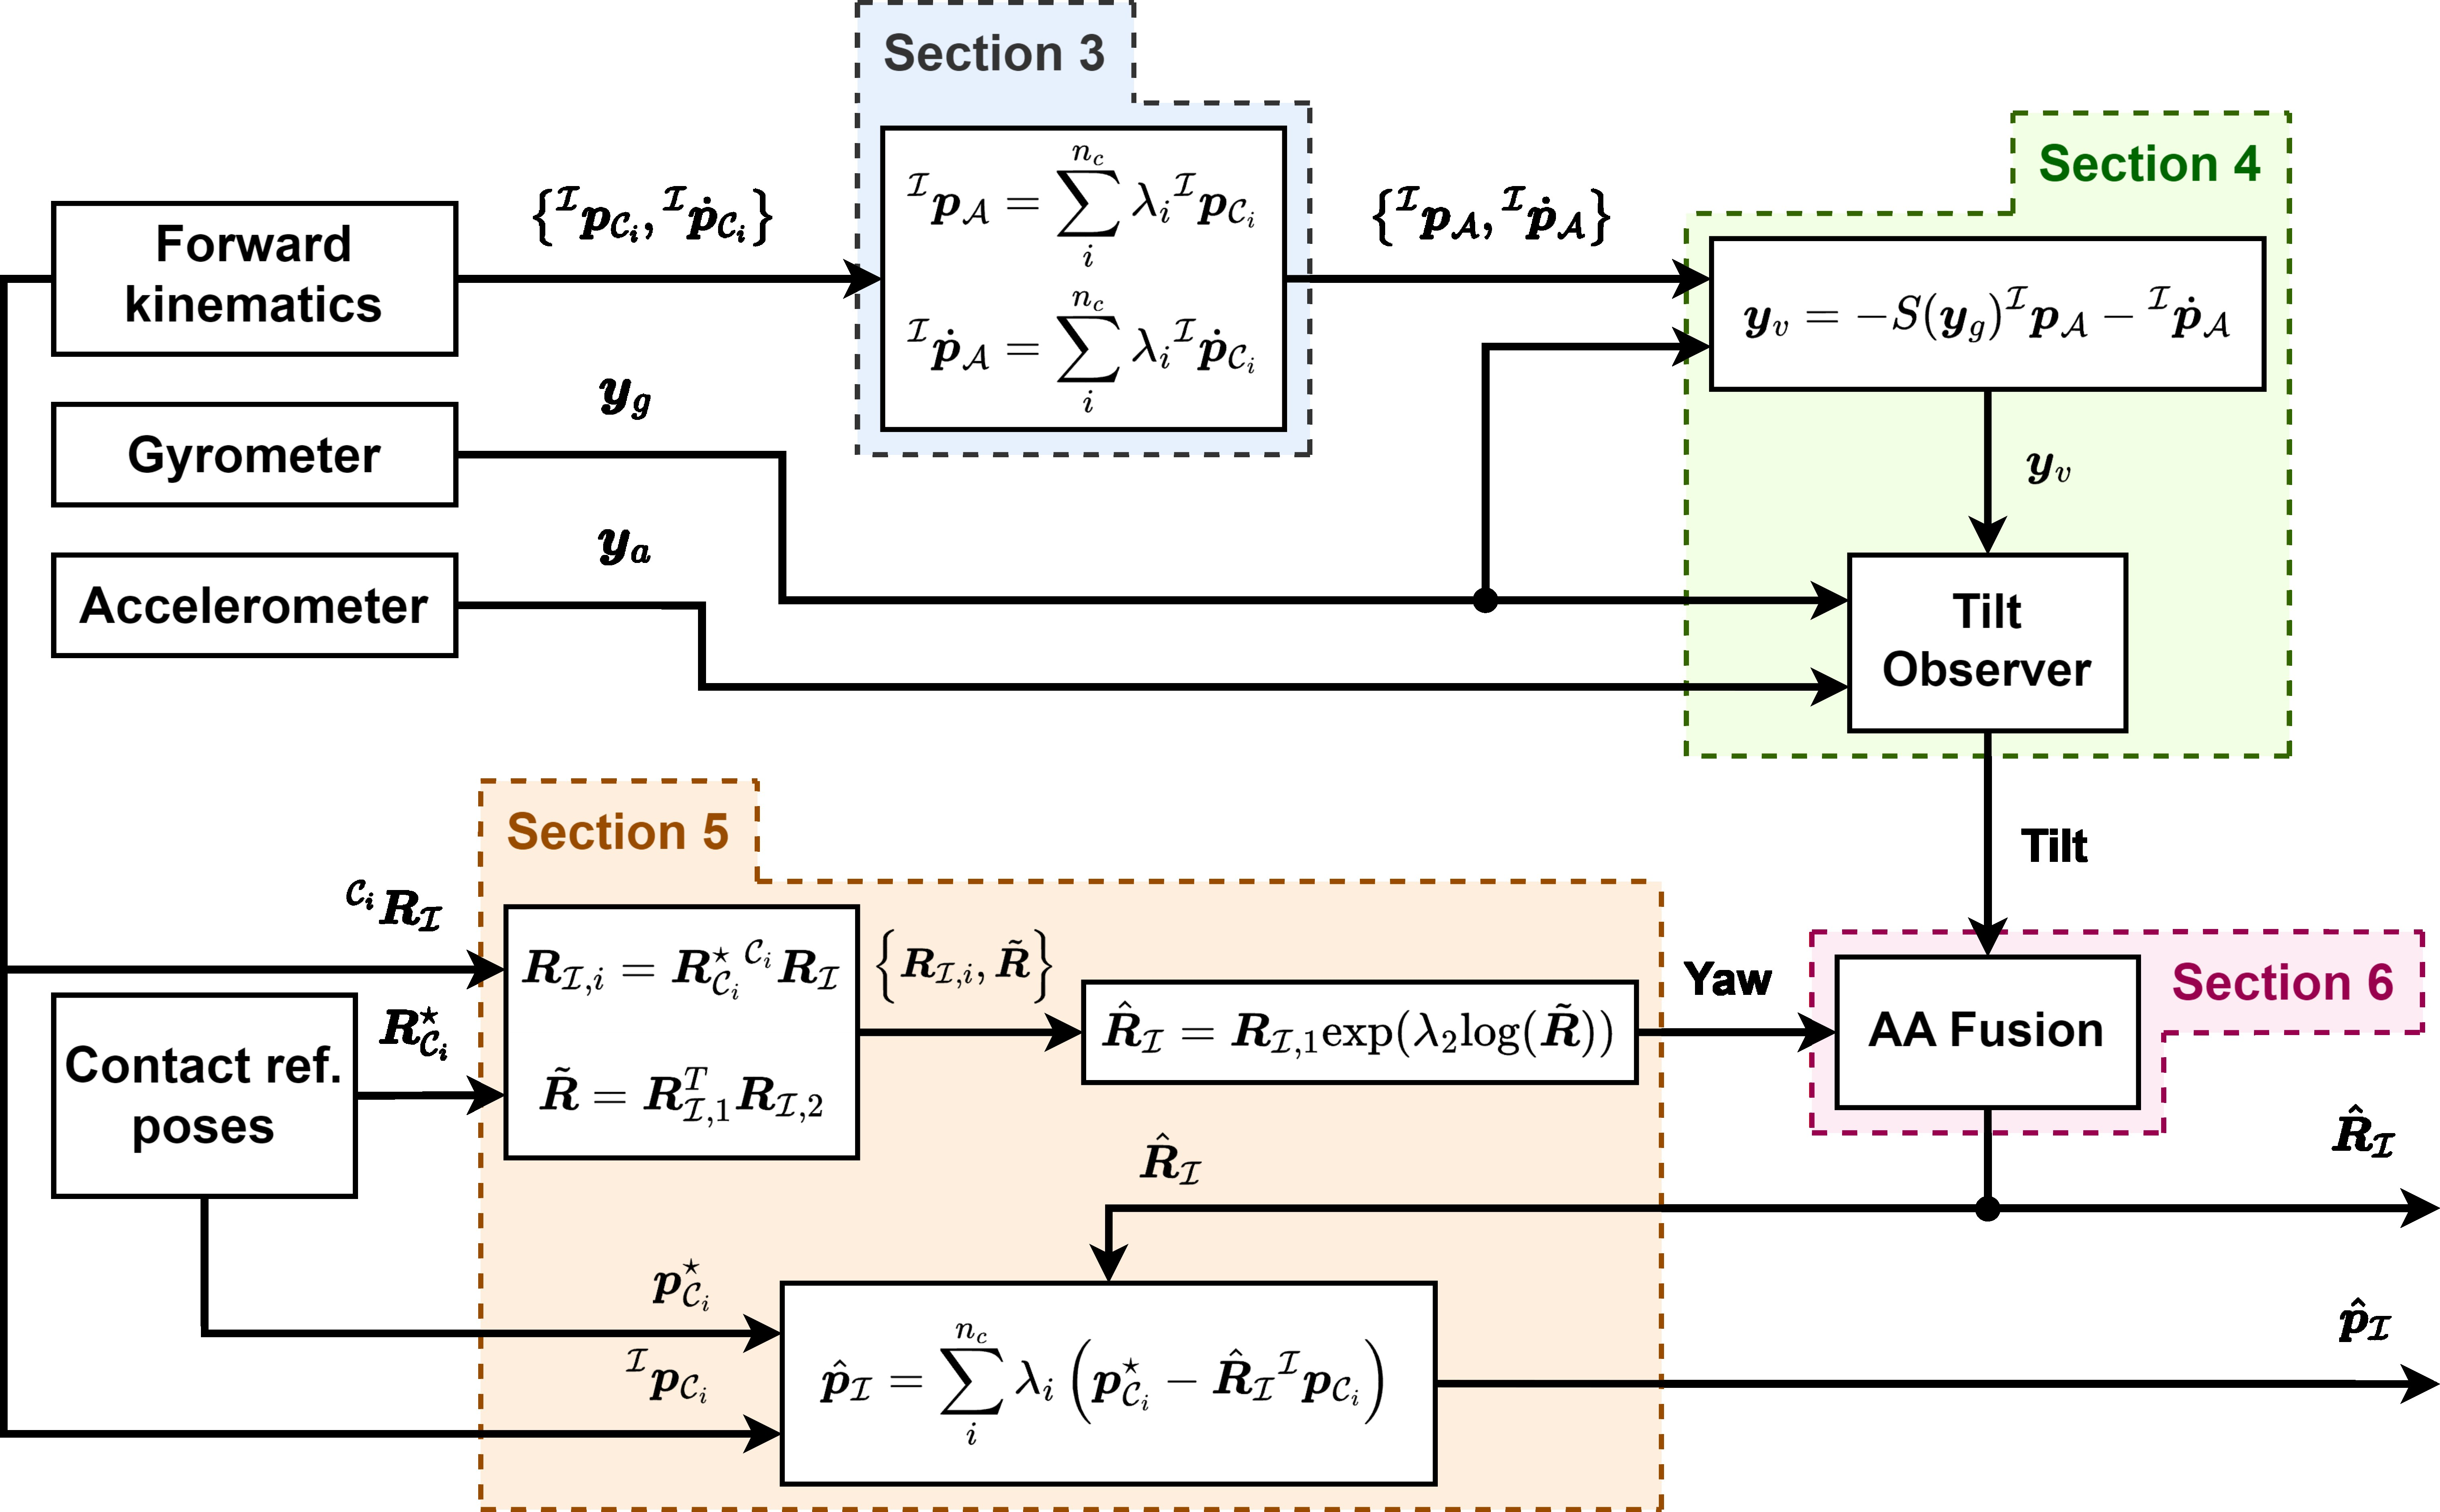
\includegraphics[width=0.90\textwidth]{Uploaded/summary.jpg}
\caption{\label{fig:summary}Summary of {\scshape Valinor}'s pipeline.}
\end{center}
\end{figure*}
 


\section{Tilt Observer with Proof of Convergence} \label{sec:Tilt}
The robot's tilt is estimated by the \emph{Tilt Observer}, which relies on the signals from an IMU and on a linear velocity measurement. Since humanoid robots are generally not equipped with a direct sensor for linear velocity, we first explain how such a measurement can be reconstructed in the case of legged robot.

\subsection{Linear velocity pseudo-measurement}
The pseudo-measurement is obtained using the so-called \emph{anchor point}, a point rigidly attached to the robot whose velocity in the world frame is assumed to be zero. Under the common assumption that legged robot contacts remain fixed in the world, any point on a contact surface could serve as an anchor point. However, this assumption may be violated in the presence of slippage. To make the zero-velocity assumption as robust as possible, we compute the anchor point as a weighted average of all contact positions, assigning greater weight to those less prone to slip. Specifically, for each contact $i$, we calculate a coefficient $u_i$ from the measured contact force $\boldsymbol{F}_{i}$, quantifying its slip susceptibility according to Coulomb's law: 
\begin{equation}
    u_{i} = \frac{F_{i,z}}{\sqrt{F_{i,x}^2 + F_{i,y}^2} + \epsilon mg_{0}},\label{eq:ratio_ui}
\end{equation}
with $mg_{0}$ the weight of the robot, and $\epsilon$, an arbitrarily small term, which allows to deal with the case where the tangential force is zero. \\
We then normalize the coefficients to obtain $\lambda_i$ for each contact, which are subsequently used to weight their contributions in the average:
\begin{equation}
    \lambda_{i}=\frac{u_{i}}{\sum^{n_{c}}_{j=1}u_{j}}. \label{eq:lambda_i}
\end{equation}
Based on the definition of the anchor point, we give its position and linear velocity in the IMU's frame:
\begin{equation} 
{^{\mathcal{I}}}\boldsymbol{p}_{\mathcal{A}} = \sum^{n_{c}}_{i} \lambda_{i}  {^{\mathcal{I}}} \boldsymbol{p}_{{\mathcal{C}}_{i}} , \qquad \qquad {^{\mathcal{I}}} \dot{\boldsymbol{p}}_{\mathcal{A}} = \sum^{n_{c}}_{i} \lambda_{i}  {^{\mathcal{I}}} \dot{\boldsymbol{p}}_{{\mathcal{C}}_{i}}, \label{eq:imuAnchorKine} 
\end{equation} 
with ${^{\mathcal{I}}} \boldsymbol{p}_{{\mathcal{C}}_{i}}$ the position and ${^{\mathcal{I}}} \dot{\boldsymbol{p}}_{{\mathcal{C}}_{i}}$ the linear velocity of the $i$-th contact in the IMU's frame, which are directly provided by the robot's joint encoders and geometrical model.

Finally, we construct a pseudo-measurement $\boldsymbol{y}_v$ of the IMU's linear velocity in the world (expressed in the IMU frame) from the gyrometer signal $\boldsymbol{y}_g$, together with the anchor point's position and velocity in the IMU frame and its assumed zero velocity in the world:
\begin{equation}
    \boldsymbol{y}_v = - \boldsymbol{y}_{g} \times {^{\mathcal{I}}}\boldsymbol{p}_{\mathcal{A}} - {^{\mathcal{I}}} \dot{\boldsymbol{p}}_{\mathcal{A}} \label{eq:yv}
\end{equation}


\subsection{Definition of the Tilt Observer}
The Tilt Observer provides estimates of: 
\begin{itemize}
    \item $\boldsymbol{v}_{\mathcal{I}, \text{l}} \triangleq \boldsymbol{R}^{T}_{\mathcal{I}} \boldsymbol{v}_{\mathcal{I}} $ the linear velocity of the IMU's frame in the world frame, expressed in the frame of the IMU.
    \item $\boldsymbol{R}^{T}_{\mathcal{I}} \boldsymbol{e}_z$ the tilt of the IMU.
\end{itemize}
We thus define the state variables: 
\begin{alignat}{2}
&\boldsymbol{x}_{1} \triangleq \boldsymbol{v}_{\mathcal{I}, \text{l}} \quad &&, \boldsymbol{x}_{1} \in \mathbb{R}^{\text{3}}, \label{eq:x1} \\
&\boldsymbol{x}_{2} \triangleq \boldsymbol{R}^{T}_{\mathcal{I}} \boldsymbol{e}_z \quad &&, \boldsymbol{x}_{2} \in \mathbb{S}^{\text{2}}. \label{eq:x2}
\end{alignat} 
The set $\mathbb{S}^{\text{2}} \subset \mathbb{R}^{\text{3}}$ is the unit sphere centered at the origin, and defined as $\mathbb{S}^{\text{2}} = \left\{ \boldsymbol{x} \in \mathbb{R}^{\text{3}} \vert \lVert \boldsymbol{x} \rVert=\text{1} \right\}$.
The Tilt Observer consists in a complementary filter, which uses the system's dynamics as a feed-forward, and corrects the estimated state using the velocity measurement $\boldsymbol{y}_{v}$:
\begin{empheq}[left= \empheqlbrace]{align}
    \dot{\hat{\boldsymbol{x}}}_{1} &= - \boldsymbol{y}_{g} \times \hat{\boldsymbol{x}}_{1} - g_{0} \hat{\boldsymbol{x}}_{2}^{\prime} + \boldsymbol{y}_{a} + \alpha_{1} (\boldsymbol{y}_{v} - \hat{\boldsymbol{x}}_{1}) \text{, }\label{eq:tilt_dynamics_1} \\
    \dot{\hat{\boldsymbol{x}}}_{2}^{\prime} &= -  \boldsymbol{y}_{g} \times \hat{\boldsymbol{x}}_{2} - \frac{\alpha_{2}}{g_{0}} (\boldsymbol{y}_{v} - \hat{\boldsymbol{x}}_{1}) \text{, }\label{eq:tilt_dynamics_2} \\
    \dot{\hat{\boldsymbol{x}}}_{2} &= - (\boldsymbol{y}_{g} - \gamma \hat{\boldsymbol{x}}_{2} \times \hat{\boldsymbol{x}}_{2}^{\prime})\times \hat{\boldsymbol{x}}_{2} \text{. } \label{eq:tilt_dynamics_3}
\end{empheq}
$\hat{\boldsymbol{x}}_{1} $ is the estimate of $\boldsymbol{x}_{1} $ and $\hat{\boldsymbol{x}}_{2}^{\prime}$ is an intermediate estimate of $\boldsymbol{x}_{2} $, which converges exponentially, but is not restricted to lie on the sphere $\mathbb{S}^{\text{2}}$. This estimate drives the convergence of the tilt's final estimate $\hat{\boldsymbol{x}}_{2} $, which is explicitly projected onto $\mathbb{S}^{\text{2}}$ so as to respect its Lie group structure.
The positive scalar gains $\alpha_1$, $\alpha_2$ and $\gamma$ define the convergence rates of the three state estimates. Insights on their tuning are provided in~\cite{benallegue2023velocity}. 

The formulation as a complementary filter allows to conduct a convergence analysis of the estimation error, providing strong mathematical guarantees on the estimator's performances. Especially here, it has been shown in~\cite{benallegue2020LyapunovStableOrientationEstimatorHumanoids} that:
\begin{itemize}
    \item The dynamics of the estimation error is autonomous, and thus does not depend on the motion of the robot. 
    \item The intermediate estimator $\left\{\hat{\boldsymbol{x}}_{1}, \hat{\boldsymbol{x}}_{2}^{\prime} \right\}$ is \emph{globally exponentially stable}, with respect to the origin $\left(0,0\right)$.
    \item The full estimator is \emph{almost globally asymptotically stable}, and locally \emph{exponentially stable}. It provides a good filtering of noise and guarantees to respect the normality constraint.
\end{itemize}
Note that the filter's convergence guarantees hold regardless of the gains' tuning.

\section{Leg Odometry for Position and Yaw Estimation}\label{sec:Leg_odom}

While the tilt of the IMU's frame in the world frame is estimated by the Tilt Observer, its position and yaw are obtained using Leg odometry. Once a contact is created, its initial pose in the world is obtained by forward kinematics from the current IMU's frame pose and the robot's joint encoders. We call it the contact's \emph{reference} pose $\left\{ \boldsymbol{p}^{\star}_{\mathcal{C}}, \boldsymbol{R}^{\star}_{\mathcal{C}}\right\}$, which we consider constant to enforce the contact's anchoring role. This pose is then used to recover the pose of the IMU's frame in the world frame. 
With the proposed pipeline, we thus leverage both the accuracy and mathematical guarantees provided by the Tilt Observer, and the robustness to drift provided by the Leg odometry. Similarly to the computation of the anchor point, the contribution of contacts to the Leg odometry is weighted to trust more contacts which are the least prone to slippage, in order to mitigate its effect.

\section{Tilt--Yaw Fusion}
The Tilt Observer provides an accurate
estimate of the IMU \emph{tilt}
\(
  \boldsymbol{\ell}=\boldsymbol{R}_{1}^{\top}\boldsymbol{e}_{z},
\)
while the contact–based Leg odometry supplies an orientation \(\boldsymbol{R}_{2}\) whose
yaw reflects the robot heading.  We now merge these two pieces into a
single rotation \(\boldsymbol{R}\).

Classically in these situations, the Euler angles representation of the rotations would be used. 
Despite the simplicity of this method, its rests on two tacit assumptions that are seldom met in the Leg–Inertial setting considered
here:

\begin{itemize}
\item The optimality of this fusion is defined with
      respect to the IMU axis $\boldsymbol{e}_{x}$ only.  
      This makes sense when $\boldsymbol{e}_{x}$ \emph{is} the heading
      carrier, for example with a GPS-based heading for wheeled vehicles.  
      In practice the IMU can be installed with an arbitrary yaw
      offset, and our yaw information actually comes from Leg odometry (average contact frames), not from
      that axis.  Treating $\boldsymbol{e}_{x}$ as ``special'' therefore
      introduces a systematic bias.

\item Because this fusion uses a ZYX decomposition of
      $\boldsymbol{R}_{1}$, it inherits the Euler-angle singularity at
      $\theta_{1}= \pm 90^{\circ}$.  
      Exactly there the pitch axis aligns with
      $\boldsymbol{e}_{z}$, roll and yaw collapse, and the horizontal
      projection of $\boldsymbol{e}_{x}$ disappears, leaving the yaw
      numerically indeterminate.  
      Such attitudes are frequent in humanoids that perform
      multicontact motions.
\end{itemize}

To avoid these two issues we adopt an \emph{axis-agnostic} fusion of tilt and yaw that
uses solely the measured tilt $\boldsymbol{\ell}$ and allows any horizontal
vector to encode yaw.

\section{Experimental Evaluation}

The proposed estimator has been compared to the state-of-the-art RI-EKF~\cite{Hartley2020RIEKF}, accross two experimental scenarios on two different humanoid robots:
\begin{itemize}
    \item Experiment 1: A walk on a flat ground over about 18 meters with the robot RHP Friends. This experiment was repeated 5 times, for a total distance of about 90 meters.
    \item Experiment 2: A multi-contact motion over about 2 meters with the robot HRP-5P. This motion involved an additional contact at the robot's left hand, and non-coplanar contacts on tilted obstacles. This experiment was repeated 4 times for a total distance of about 8 meters.
\end{itemize}
\subsection{Computational Performance Evaluation}\label{subsec:computation_time}

We first evaluated the computation speed performance of the proposed estimator on a laptop with an Intel Xeon E-2176M CPU (2.70GHz x 12), over the four multi-contact experiments. In average, an iteration of {\scshape Valinor} was computed in 2.547 \textmu s, against 19.315 \textmu s for the RI-EKF. It is thus more than 7.5 times faster, while proposing equivalent estimation accuracy, or even improving the estimation of key variables, as shown in Table~\ref{tab:estimation_eval}.

\subsection{Estimation Accuracy Evaluation} ~\label{subsec:est_accur_eval}

\begin{table}[h!] 
\setlength{\extrarowheight}{0.6ex}
\addtolength{\tabcolsep}{-0.4em}
\caption{Mean and standard deviation (in parentheses) of the estimation errors during the four trials of Experiment 2. RE is the The 0.3 m Relative Error. } \label{tab:estimation_eval}
{\footnotesize
    \begin{center}
        \begin{tabu}to\linewidth{| X[c] | X[c] | X[c] | X[c] | X[c] | X[c] | X[c] |}
            \hline
                  &       \multicolumn{2}{c|}{RE Translation}         &    \multicolumn{2}{c|}{RE Orientation}  &    \multicolumn{2}{c|}{Linear velocity}     \\     

            &       \multicolumn{2}{c|}{[m]}         &    \multicolumn{2}{c|}{ [\textdegree] }  &    \multicolumn{2}{c|}{[$\text{m/s}$]}     \\     
                  
            \cline{2-7}
              &     Lateral    &      Vertical      &   \multirow{2}{*}{Tilt}      &     \multirow{2}{*}{Yaw}    &  Lateral  &  Vertical \\ 
              &    \{$\boldsymbol{x}, \boldsymbol{y}$\}    &     $\boldsymbol{z}$      &      &      &   \{$\boldsymbol{x}, \boldsymbol{y}$\}  &  $\boldsymbol{z}$ \\
            \hline     
            \multirow{2}{*}{Ours}  &  \textbf{\getErrorResult{Multicontact}{Tilt}{Relerror}{Transxy}{Meanabs}}  &  \textbf{\getErrorResult{Multicontact}{Tilt}{Relerror}{Transz}{Meanabs}}   &    \textbf{\getErrorResult{Multicontact}{Tilt}{Relerror}{Tilt}{Meanabs}}    &    \textbf{\getErrorResult{Multicontact}{Tilt}{Relerror}{Yaw}{Meanabs}}     &  \getErrorResult{Multicontact}{Tilt}{Velerror}{EstimateXy}{Meanabs}    &   \textbf{\getErrorResult{Multicontact}{Tilt}{Velerror}{EstimateZ}{Meanabs}}  \\ 
               &  (\getErrorResult{Multicontact}{Tilt}{Relerror}{Transxy}{Std})   &      (\getErrorResult{Multicontact}{Tilt}{Relerror}{Transz}{Std})      &   (\getErrorResult{Multicontact}{Tilt}{Relerror}{Tilt}{Std})   &     (\getErrorResult{Multicontact}{Tilt}{Relerror}{Yaw}{Std})   &  (\getErrorResult{Multicontact}{Tilt}{Velerror}{EstimateXy}{Std})   &   (\getErrorResult{Multicontact}{Tilt}{Velerror}{EstimateZ}{Std})  \\ 
            \hline
            RI-EKF  &  \getErrorResult{Multicontact}{Hartley}{Relerror}{Transxy}{Meanabs}  &   \getErrorResult{Multicontact}{Hartley}{Relerror}{Transz}{Meanabs}   &    \getErrorResult{Multicontact}{Hartley}{Relerror}{Tilt}{Meanabs}    &    \getErrorResult{Multicontact}{Hartley}{Relerror}{Yaw}{Meanabs}   &  \textbf{\getErrorResult{Multicontact}{Hartley}{Velerror}{EstimateXy}{Meanabs}}    &   \getErrorResult{Multicontact}{Hartley}{Velerror}{EstimateZ}{Meanabs}  \\ 
            \cite{Hartley2020RIEKF} & (\getErrorResult{Multicontact}{Hartley}{Relerror}{Transxy}{Std})    &     (\getErrorResult{Multicontact}{Hartley}{Relerror}{Transz}{Std})    &     (\getErrorResult{Multicontact}{Hartley}{Relerror}{Tilt}{Std})   &    (\getErrorResult{Multicontact}{Hartley}{Relerror}{Yaw}{Std})    &  (\getErrorResult{Multicontact}{Hartley}{Velerror}{EstimateXy}{Std})    &   (\getErrorResult{Multicontact}{Hartley}{Velerror}{EstimateZ}{Std})  \\ 
            \hline     
        \end{tabu}
    \end{center}
}
\end{table}

These results show that {\scshape Valinor} improved the estimation of lateral translations by over 40\% compared to the RI-EKF, and improved that of the robot's tilt by 60\%. For both translations and tilt estimates, our method displayed a significantly lower standard deviation of the error, proving an improved estimation consistency. 


%%%%%%%%%%%%%%%%% BIBLIOGRAPHY IN THE LaTeX file !!!!! %%%%%%%%%%%%%%%%%%%%%%
%%---------------------------------------------------------------------------%%
%
% \begin{thebibliography}{99}

% \bibitem{ref1}
% J. H. Bong, ``Controlling the parasite,'' in \textit{Proc. of International Conference on Control, Automation and Systems}, pp. 0209-0210, 2020


% \bibitem{ref2}
% A. Alice and B. Bob, ``Nonlinear unstable systems,'' \textit{International Journal of Control, Automation, and Systems}, vol. 23, no. 4, pp. 123–145, 1989.

% \bibitem{ref3}
% M. Young, \textit{The Technical Writer's Handbook}, Mill Valley, Seoul, 1989.



% \end{thebibliography}
% %
% %%--------------------------------------------------------------------%%

\bibliographystyle{IEEEtran}
\bibliography{IEEEabrv, Uploaded/Bibliography}

\end{document}
